% !TXS template
\documentclass[titlepage]{article}
\usepackage[utf8]{inputenc}
\usepackage{color}   %May be necessary if you want to color links
\usepackage{hyperref}
\usepackage[french]{babel}
\usepackage{cite}
\usepackage{graphicx}

\hypersetup{
	colorlinks=true, %set true if you want colored links
	linktoc=all,     %set to all if you want both sections and subsections linked
	linkcolor=blue,  %choose some color if you want links to stand out
}
\title{Arbre comportementaux pour le contr\^ole de mission}
\author{
	Derrien Martial \\
	\and
	Madec Antoine \\
	\and
	Lucas Florian
}
\date{Juin 2019}
\renewcommand{\contentsname}{Sommaire} 
\begin{document}
	\maketitle
	\tableofcontents
	\hypersetup{linktocpage}
	
	\clearpage
	\part{Introduction}
	Un arbre comportemental (Behavior Tree, BT en anglais) est une
	technique permettant de structurer le passage d'une tâche à une autre dans 
	le cadre de l'automatisation de ce comportement. \cite{colledanchise_ogren_2018}
	\\
	\begin{figure}[h!]
		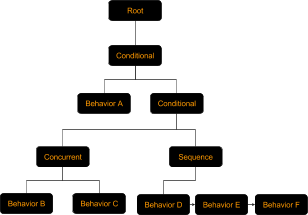
\includegraphics[width=\linewidth]{img/behavior_trees_example.png}
		\caption{A boat.}
		\label{fig:boat1}
	\end{figure}
	\\
	d’intelligence artificielle dérivée de l’algorithme des arbres
	de décision. \cite{rasmussen}
	Cet algorithme, très utilisé dans le domaine des jeux
	vidéo depuis déjà de nombreuses années, commence a être utilisée en
	robotique pour le contrôle de systèmes de plus en plus complexes.\cite{ros.org}
	
	\clearpage
	\part{Les grands domaines d'emploi des behavior trees}
	\section{Structure}
	This section's content...
	\paragraph{ceci est un paragraphe}	
	\subsection{Top Matter}
	This subsection's content...
	\subsubsection{Article Information}
	This subsubsection's content...
	
	\clearpage
	\bibliographystyle{alpha}
	\bibliography{sources.bib}
	
\end{document}
